\resizebox{\linewidth}{!}{
\begin{tikzpicture}
    % Colors definition: latexcolor.com
    \definecolor{ashgrey}{rgb}{0.7, 0.75, 0.71}
    \definecolor{x11gray}{rgb}{0.75, 0.75, 0.75}
    \definecolor{metal}{rgb}{0.43, 0.5, 0.5}
    \definecolor{blue0}{RGB}{0,25,51}
    \definecolor{blue1}{RGB}{0,51,102}
    \definecolor{blue2}{RGB}{0,128,255}
    \definecolor{blue3}{RGB}{153,204,255}
    \definecolor{yellow}{RGB}{250,165,25}
    \definecolor{lightyellow}{RGB}{229,208,66}

    
    % Main outline LHS
    % Background
    \draw[fill=blue1!50, visible on=<5->] (0, 2.75) rectangle (6.75, 6.0);

    % Client Side
    % Client boxes line
    % Client 1
    \draw[fill=gray!5] (0,1.5) rectangle (2, 2.25);
    \node at (1.6, 1.825) {
\includegraphics[width=10pt]{images/smartwatch.png}};
    \node[visible on=<4->] at (1.05, 1.825) {
\includegraphics[width=10pt]{images/wifi-signal.png}};
    \node at (0.4, 1.825) {
\includegraphics[width=15pt]{images/raspberry.png}};
    % Client 2
    \draw[fill=gray!5] (2.5,1.5) rectangle (4.5, 2.25);
    \node at (2.9, 1.825) {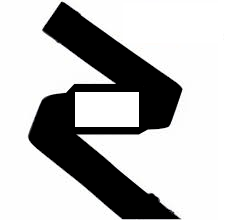
\includegraphics[width=10pt]{images/hrband.png}};
    \node[visible on=<4->] at (3.5, 1.825) {
\includegraphics[width=10pt]{images/wifi-right.png}};
    \node at (4.1, 1.825) {
\includegraphics[width=15pt]{images/raspberry.png}};
    % Client m
    \draw[fill=gray!5] (6,1.5) rectangle (6.75, 2.25) node[pos=.5] {\tiny{Client $m$}};
    % Lines to filesystem
    \draw[<->, dashed, thick, visible on=<5->] (0.4, 2.25) -- (0.4, 3.5) -- (1, 3.5);
    \draw[<->, dashed, thick, visible on=<5->] (4.1, 2.25) -- (4.1, 2.35) -- (1.35, 2.35) -- (1.35, 3);
    \draw[<->, dashed, thick, visible on=<5->] (6.3725, 2.25) -- (6.3725, 2.55) -- (1.85, 2.55) -- (1.85, 3);

    % Server Side
    % FileSystem Logo
    \draw[fill=x11gray!50, visible on=<5->] (1.0, 3) -- (1.1, 3.9) -- (1.6, 3.9) -- (1.75, 4.0) -- (2.1, 4.0) -- (2.0, 3);
    %\draw[fill=x11gray] (1.0, 3) -- (1.0, 3.8) -- (1.6, 3.8) -- (1.75, 3.6) -- (2.0, 3.6) -- (2.0, 3) -- (1.0, 3);
    \node[visible on=<5->] at (1.4, 5.0) {\text{\tiny{\textbf{FileSystem Interface}}}};
    % SGX Spark
    % Main Outline
    \draw[fill=white, visible on=<6->] (2.75, 3) rectangle (6.25, 5.5);
    \node[visible on=<6->] at (4.4, 5.7) {\text{\textbf{\tiny{SGX-Spark Engine}}}};
    % SHM
    \draw[visible on=<6->] (2.95, 3.2) rectangle (6.05, 3.5) node[pos=.5] {\tiny{Host Shared Memory}};
    % Driver
    \draw[pattern=north west lines,pattern color=yellow, visible on=<6->] (2.95, 3.7) rectangle (3.95, 4.4); 
    \node[visible on=<6->] at (3.7, 4.5) {\tiny{\texttt{driver-enclave.sh}}};
    \node[visible on=<6->] at (3.95, 3.7) {
\includegraphics[width=8pt]{images/intel-sgx.png}};
    \draw[visible on=<6->] (2.95, 4.6) rectangle (3.95, 5.3); 
    \node[visible on=<6->] at (3.35, 5.4) {\tiny{\texttt{master.sh}}};
    % Worker
    \draw[pattern=north west lines,pattern color=yellow, visible on=<6->] (4.15, 3.7) rectangle (6.05, 4.4);
    \node[visible on=<6->] at (4.9, 3.6) {\tiny{\texttt{worker-enclave.sh}}};
    \draw[visible on=<6->] (4.15, 4.6) rectangle (6.05, 5.3);
    \node[visible on=<6->] at (4.55, 5.4) {\tiny{\texttt{worker.sh}}};
    % Tasks Enclave
    \draw[fill=white, visible on=<6->] (4.25, 3.8) rectangle (4.65, 4.3) node[pos=.5] {\tiny{$T_1$}};
    \draw[fill=white, visible on=<6->] (4.75, 3.8) rectangle (5.15, 4.3) node[pos=.5] {\tiny{$T_2$}};
    \node[visible on=<6->] at (5.35, 4.05) {\tiny{$\cdots$}};
    \draw[fill=white, visible on=<6->] (5.55, 3.8) rectangle (5.95, 4.3) node[pos=.5] {\tiny{$T_N$}};
    \node[visible on=<6->] at (6, 3.7) {
\includegraphics[width=8pt]{images/intel-sgx.png}};
    % Tasks Outside Enclave
    \draw[visible on=<6->] (4.25, 4.7) rectangle (4.65, 5.2) node[pos=.5] {\tiny{$T_1$}};
    \draw[visible on=<6->] (4.75, 4.7) rectangle (5.15, 5.2) node[pos=.5] {\tiny{$T_2$}};
    \node[visible on=<6->] at (5.35, 4.95) {\tiny{$\cdots$}};
    \draw[visible on=<6->] (5.55, 4.7) rectangle (5.95, 5.2) node[pos=.5] {\tiny{$T_N$}};

    % CSEM's Toolbox
    \draw[fill=white, visible on=<5->] (0.9, 3.7) rectangle (2.0, 4.75);
    \node[visible on=<5->] at (1.45, 4.55) {\textbf{\tiny{CSEM HRV}}};
    \draw[dashed, visible on=<5->] (0.9, 4.4) -- (2.0, 4.4);
    \node[visible on=<5->] at (1.45, 4.25) {\texttt{\tiny{+ Identity}}};
    \node[visible on=<5->] at (1.28, 4.05) {\texttt{\tiny{+ SDNN}}};
    \node[visible on=<5->] at (1.46, 3.85) {\texttt{\tiny{+ HRVBands}}};
    \draw[fill=x11gray, visible on=<5->] (1.0, 3) -- (1.0, 3.8) -- (1.6, 3.8) -- (1.75, 3.6) -- (2.0, 3.6) -- (2.0, 3) -- (1.0, 3);

    %% LHS - Workflow Storyline
    % Separator
    \draw (7.3, 1.5) -- (7.3, 6);
    \draw (7.5, 1.5) -- (7.5, 6);

    % Stage 2: Client Breakdown
    \draw[fill=blue1!70, visible on=<2>] (8, 2.75) rectangle (10.5, 5.55);
    %\draw (9.25, 1.3725) circle (0.5);
    \draw[dashed, visible on=<2>] (8, 3.55) -- (10.5, 3.55);
    \draw[fill=white, visible on=<2>] (8.2, 2.95) rectangle (10.3, 3.35) node[pos=.5] {\tiny{\texttt{sensor}}};
    \node[visible on=<2>] at (10.3, 3.00) {
\includegraphics[width=10pt]{images/docker.png}};
    \node[visible on=<2>] at (8.2, 3.00) {
\includegraphics[width=8pt]{images/smartwatch.png}};
    \draw[fill=white, visible on=<2>] (8.2, 3.75) rectangle (10.3, 4.15) node[pos=.5] {\tiny{\texttt{eclipse-mqtt}}};
    \node[visible on=<2>] at (10.3, 3.80) {
\includegraphics[width=10pt]{images/docker.png}};
    \draw[fill=white, visible on=<2>] (8.2, 4.35) rectangle (10.3, 4.75) node[pos=.5] {\tiny{\texttt{mqtt-subscriber}}};
    \node[visible on=<2>] at (10.3, 4.40) {
\includegraphics[width=10pt]{images/docker.png}};
    \draw[fill=white, visible on=<2>] (8.2, 4.95) rectangle (9.2, 5.35) node[pos=.5] {\tiny{\texttt{consumer}}};
    \node[visible on=<2>] at (8.3, 5.00) {
\includegraphics[width=10pt]{images/docker.png}};
    \draw[fill=white, visible on=<2>] (9.3, 4.95) rectangle (10.3, 5.35) node[pos=.5] {\tiny{\texttt{producer}}};
    \node[visible on=<2>] at (10.3, 5.00) {
\includegraphics[width=10pt]{images/docker.png}};
    \draw[->, very thick, dashed, visible on=<2>] (9.8, 5.35) -- (9.8, 6);
    \draw[<-, very thick, dashed, visible on=<2>] (8.7, 5.35) -- (8.7, 6);
    % Client box below
    \node at (5.265, 1.85) {$\cdots$};
    \draw[fill=gray!5, visible on=<2>] (8.875,1.5) rectangle (9.625, 2.25) node[pos=.5] {\tiny{Client}};
    \draw[dashed, thin, visible on=<2>] (8.875, 2.25) -- (8, 2.75);
    \draw[dashed, thin, visible on=<2>] (9.625, 2.25) -- (10.5, 2.75);

    % Stage 3: execution breakdown
    \node[visible on=<3->] (text-box) at (9.25,3.75) [fill=lightyellow!40,minimum width=2.75cm,minimum height=4.5cm] {};
    % Title:
    \node[anchor=north west, visible on=<3>,align=left] (text) at (text-box.north west) {\textbf{\tiny{Execution Flow}}};
    % Sensors generate data and streams it to the server
    \node[anchor=north west, visible on=<4>,align=left] (text) at (text-box.north west) 
        {\textbf{\tiny{Execution Flow}} \\ 
        \setlength{\fboxrule}{0pt}
        \hspace*{-13pt}\framebox{
            {\begin{varwidth}{2.75cm}\tiny{\begin{enumerate}
                \item[\tiny{\blackcircled{1}}] \textcolor{fgRed}{Sensor} generates samples and streams them to the \textcolor{fgRed}{gateway} over \texttt{mqtt} 
            \end{enumerate}}\end{varwidth}}}
        };
    % Gateway encrypts it and sends it over
    \node[anchor=north west, visible on=<5>,align=left] (text) at (text-box.north west) 
        {\textbf{\tiny{Execution Flow}} \\ 
        \setlength{\fboxrule}{0pt}
        \hspace*{-13pt}\framebox{
            {\begin{varwidth}{2.75cm}\tiny{\begin{enumerate}
                \item[\tiny{\blackcircled{1}}] \textcolor{fgRed}{Sensor} generates samples and streams them to the \textcolor{fgRed}{gateway} over \texttt{mqtt} 
                \item[\tiny{\blackcircled{2}}] \textcolor{fgRed}{Gateway} aggregates data, encrypts it and sends it to the \textcolor{fgRed}{server}'s filesystem interface over SFTP
            \end{enumerate}}\end{varwidth}}}
        };
    % SGX-Spark Streaming Job Monitors FS, batch-processes data and saves an encrypted result in the FS
    \node[anchor=north west, visible on=<6>,align=left] (text) at (text-box.north west) 
        {\textbf{\tiny{Execution Flow}} \\ 
        \setlength{\fboxrule}{0pt}
        \hspace*{-13pt}\framebox{
            {\begin{varwidth}{2.75cm}\tiny{\begin{enumerate}
                \item[\tiny{\blackcircled{1}}] \textcolor{fgRed}{Sensor} generates samples and streams them to the \textcolor{fgRed}{gateway} over \texttt{mqtt} 
                \item[\tiny{\blackcircled{2}}] \textcolor{fgRed}{Gateway} aggregates data, encrypts it and sends it to the \textcolor{fgRed}{server}'s filesystem interface over SFTP
                \item[\tiny{\blackcircled{3}}] \textcolor{fgRed}{\texttt{SGX-Spark}} streaming job monitors the FS, \textcolor{fgRed}{batch-processes} data, and saves encrypted results back in the FS
            \end{enumerate}}\end{varwidth}}}
        };
    % Gateway periodically fetches result files from the server's filesystem
    \node[anchor=north west, visible on=<7>,align=left] (text) at (text-box.north west) 
        {\textbf{\tiny{Execution Flow}} \\ 
        \setlength{\fboxrule}{0pt}
        \hspace*{-13pt}\framebox{
            {\begin{varwidth}{2.75cm}\tiny{\begin{enumerate}
                \item[\tiny{\blackcircled{1}}] \textcolor{fgRed}{Sensor} generates samples and streams them to the \textcolor{fgRed}{gateway} over \texttt{mqtt} 
                \item[\tiny{\blackcircled{2}}] \textcolor{fgRed}{Gateway} aggregates data, encrypts it and sends it to the \textcolor{fgRed}{server}'s filesystem interface over SFTP
                \item[\tiny{\blackcircled{3}}] \textcolor{fgRed}{\texttt{SGX-Spark}} streaming job monitors the FS, \textcolor{fgRed}{batch-processes} data, and saves encrypted results back in the FS
                \item[\tiny{\blackcircled{4}}] \textcolor{fgRed}{Gateway} periodically fetches result files from the \textcolor{fgRed}{server}'s FS
            \end{enumerate}}\end{varwidth}}}
        };

\end{tikzpicture}}
